\documentclass[12pt, twoside]{book}
%\documentclass[12pt, oneside]{book}  % jednostranna tlac
\usepackage[a4paper,top=2.5cm,bottom=2.5cm,left=3.5cm,right=2cm]{geometry}
\usepackage[utf8]{inputenc}
\usepackage[T1]{fontenc}
\usepackage{graphicx}
\usepackage{url}
\usepackage[hidelinks,breaklinks]{hyperref}
\usepackage{float}
\usepackage[slovak]{babel} % vypnite pre prace v anglictine

%\let\negmedspace\relax
%\let\endnegmedspace\relax
%\let\negthickspace\relax
%\let\endnegthickspace\relax

\usepackage{amsfonts} 
\usepackage{hyperref}
\usepackage{listings}
\lstset{language=Python}
\usepackage{amsthm}

%\usepackage{algorithm}
\usepackage{algpseudocode}
\usepackage{algorithmicx}
\usepackage[noend]{algcompatible}
\usepackage{tikz}

\usepackage{mathtools}
\DeclarePairedDelimiter\ceil{\lceil}{\rceil}
\DeclarePairedDelimiter\floor{\lfloor}{\rfloor}

\newtheorem{definition}{Definícia}[chapter]
\newtheorem{theorem}[definition]{Veta}
\newtheorem{note}[definition]{Poznámka}
\newtheorem{consequence}[definition]{Dôsledok}
\newtheorem{hypothesis}[definition]{Hypotéza}
\newtheorem{alg}[definition]{Algoritmus}
\newtheorem{result}[definition]{Výsledok}
\newtheorem{lemma}[definition]{Lema}
\newtheorem{code}[definition]{Pseudokód}

%\newtheorem{subdefinition}{Definícia}[subsection]
%\newtheorem{subtheorem}{Veta}[subsection]
%\newtheorem{subnote}{Poznámka}[subsection]
%\newtheorem{subconsequence}{Dôsledok}[subsection]
%\newtheorem{subhypothesis}{Hypotéza}[subsection]
%\newtheorem{subalg}{Algoritmus}[subsection]
%\newtheorem{subresult}{Výsledok}[subsection]
%\newtheorem{sublemma}{Lema}[subsection]
%\newtheorem{subcode}{Pseudokód}[subsection]


\linespread{1.25} % hodnota 1.25 by mala zodpovedat 1.5 riadkovaniu

% -------------------
% --- Definicia zakladnych pojmov
% --- Vyplnte podla vasho zadania
% -------------------
\def\mfrok{2021}
\def\mfnazov{Magické útvary}
\def\mftyp{Bakalárska práca}
\def\mfautor{Richard Bíró}
\def\mfskolitel{doc. RNDr. Ján Mazák, PhD.}

%ak mate konzultanta, odkomentujte aj jeho meno na titulnom liste
\def\mfkonzultant{tit. Meno Priezvisko, tit. }  

\def\mfmiesto{Bratislava, \mfrok}

% bioinformatici odkomentujú riadok s dvoma odbormi a iný program
\def\mfodbor{ Informatika}
%\def\mfodbor{ Informatika a Biológia } 
\def\program{ Informatika }
%\def\program{ Bioinformatika }

% Ak je školiteľ z FMFI, uvádzate katedru školiteľa, zrejme by mala byť aj na zadaní z AIS2
% Ak máte externého školiteľa, uvádzajte Katedru informatiky 
\def\mfpracovisko{ Katedra informatiky }

\begin{document}     
\frontmatter


% -------------------
% --- Obalka ------
% -------------------
\thispagestyle{empty}

\begin{center}
\sc\large
Univerzita Komenského v Bratislave\\
Fakulta matematiky, fyziky a informatiky

\vfill

{\LARGE\mfnazov}\\
\mftyp
\end{center}

\vfill

{\sc\large 
\noindent \mfrok\\
\mfautor
}

\cleardoublepage
% --- koniec obalky ----

% -------------------
% --- Titulný list
% -------------------

\thispagestyle{empty}
\noindent

\begin{center}
\sc  
\large
Univerzita Komenského v Bratislave\\
Fakulta matematiky, fyziky a informatiky

\vfill

{\LARGE\mfnazov}\\
\mftyp
\end{center}

\vfill

\noindent
\begin{tabular}{ll}
Študijný program: & \program \\
Študijný odbor: & \mfodbor \\
Školiace pracovisko: & \mfpracovisko \\
Školiteľ: & \mfskolitel \\
% Konzultant: & \mfkonzultant \\
\end{tabular}

\vfill


\noindent \mfmiesto\\
\mfautor

\cleardoublepage
% --- Koniec titulnej strany


% -------------------
% --- Zadanie z AIS
% -------------------
% v tlačenej verzii s podpismi zainteresovaných osôb.
% v elektronickej verzii sa zverejňuje zadanie bez podpisov
% v pracach v naglictine anglicke aj slovenske zadanie

\newpage 
\thispagestyle{empty}
\hspace{-2cm}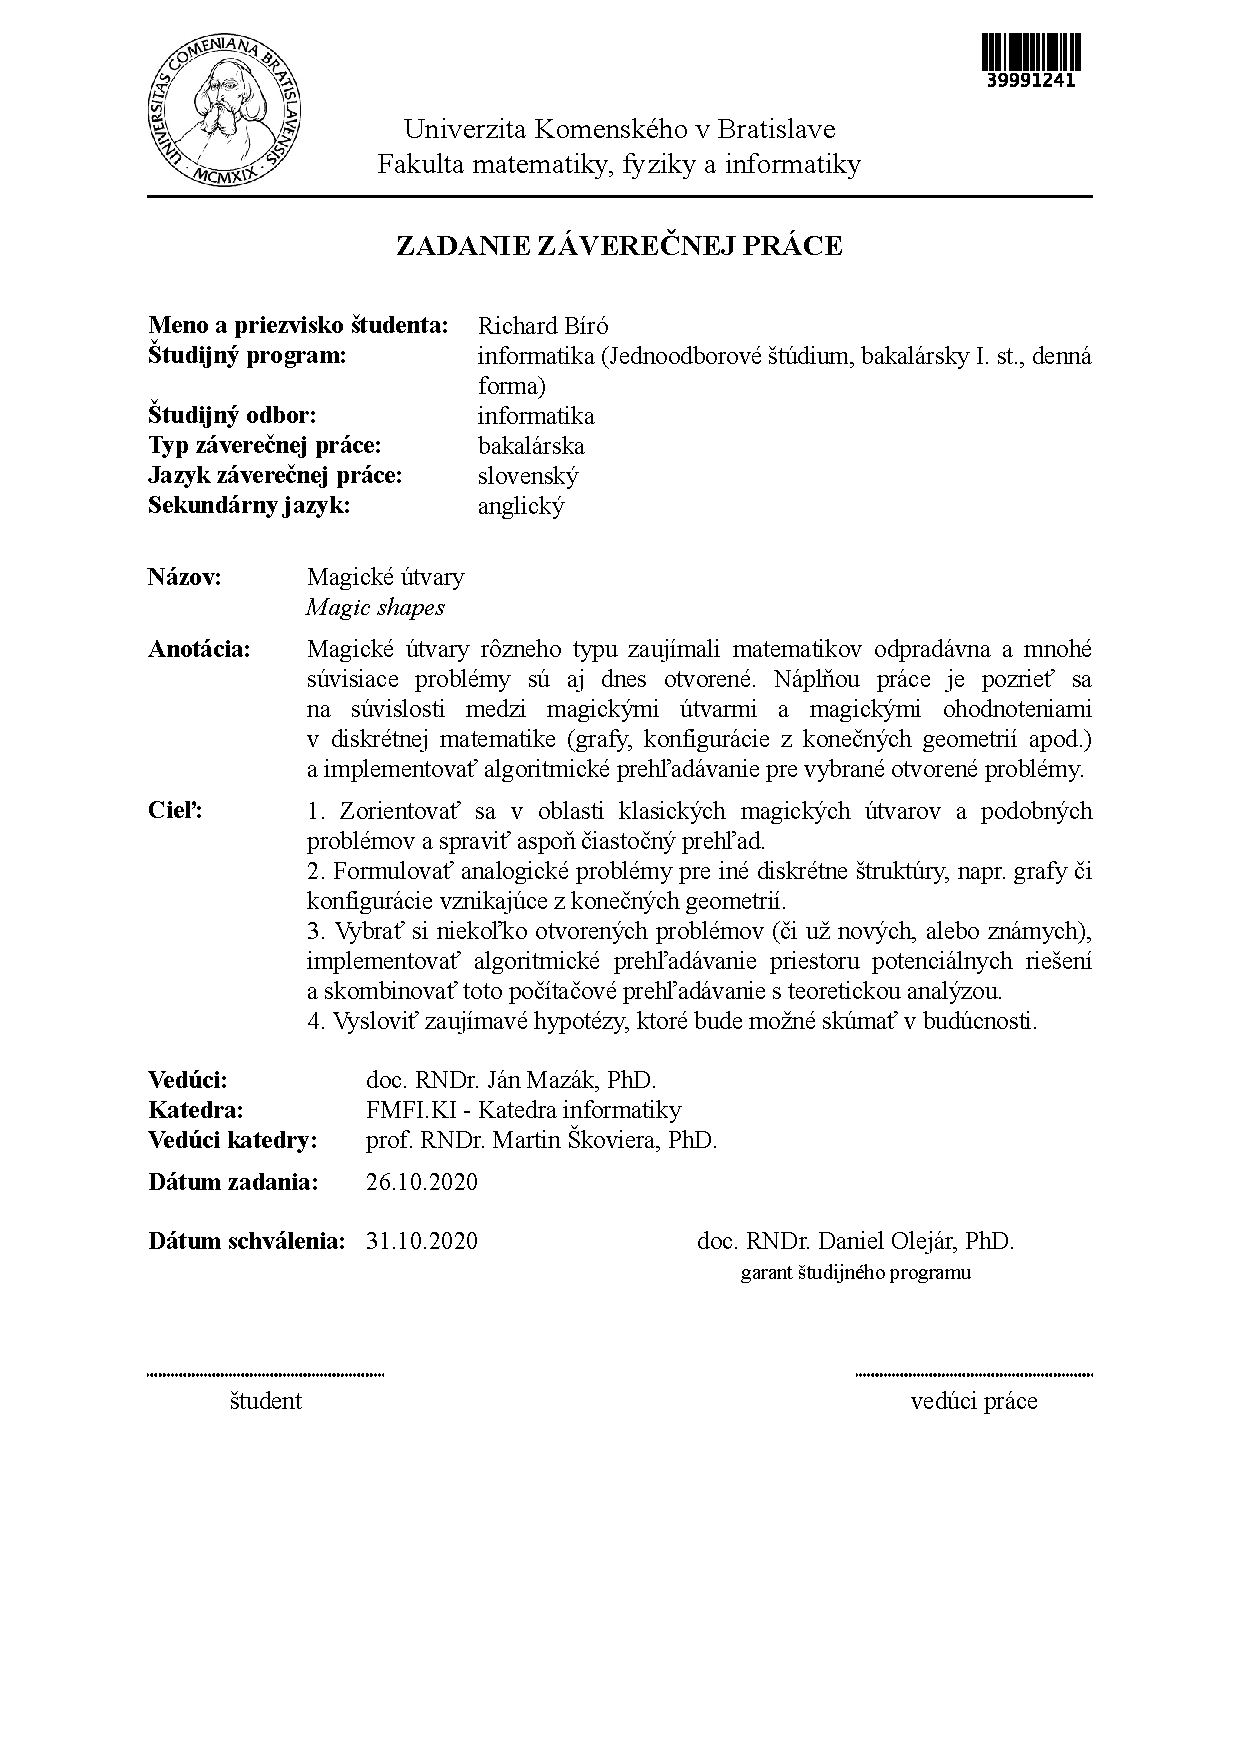
\includegraphics[width=1.1\textwidth]{images/zadanie}

% --- Koniec zadania

\frontmatter

% -------------------
%   Poďakovanie - nepovinné
% -------------------
\setcounter{page}{3}
\newpage 
~

\vfill
{\bf Poďakovanie: V prvom rade by som chcel poďakovať vedúcemu doc. RNDr. Jánovi Mazákovi, PhD. za pomoc a nápady k tejto práci. Zároveň chcem poďakovať rodičom a príbuzným za podporu. } 

% --- Koniec poďakovania

% -------------------
%   Abstrakt - Slovensky
% -------------------
\newpage 
\section*{Abstrakt}

Práca obsahuje prehľad v oblasti klasických magických útvarov. Definujeme pojmy, na základe ktorých preskúmame nové magické vlastnosti jednotlivých útvarov. Súčasťou práce je aj implementácia algoritmov na hľadanie potenciálnych riešení vybraných otvorených problémov. \\

\textbf{Kľúčové slová}: magický útvar, prvok, algoritmus

% --- Koniec Abstrakt - Slovensky

% -------------------
% --- Abstrakt - Anglicky 
% -------------------
\newpage 
\section*{Abstract}

Thesis contains overview of classic magic shapes. We explore new magic properties on the basis of our defined concepts. We also implement algoritms which look for potential solutions to chosen open problems. \\

\textbf{Keywords}: magic shape, item, algorithm

% --- Koniec Abstrakt - Anglicky

% -------------------
% --- Predhovor - v informatike sa zvacsa nepouziva
% -------------------
%\newpage 
%\thispagestyle{empty}
%
%\huge{Predhovor}
%\normalsize
%\newline
%Predhovor je všeobecná informácia o práci, obsahuje hlavnú charakteristiku práce 
%a okolnosti jej vzniku. Autor zdôvodní výber témy, stručne informuje o cieľoch 
%a význame práce, spomenie domáci a zahraničný kontext, komu je práca určená, 
%použité metódy, stav poznania; autor stručne charakterizuje svoj prístup a svoje 
%hľadisko. 
%
% --- Koniec Predhovor


% -------------------
% --- Obsah
% -------------------

\newpage 

\tableofcontents

% ---  Koniec Obsahu

% -------------------
% --- Zoznamy tabuliek, obrázkov - nepovinne
% -------------------

\newpage 

%\listoffigures

% ---  Koniec Zoznamov

\mainmatter


\input uvod.tex 

\input kapitola1.tex

\input kapitola2.tex

\input kapitola3.tex

\input kapitola4.tex

\input zaver.tex

% -------------------
% --- Bibliografia
% -------------------


\newpage	

\backmatter

\thispagestyle{empty}
\clearpage

\bibliographystyle{plain}
%\bibliography{literatura} 

%Prípadne môžete napísať literatúru priamo tu
\begin{thebibliography}{7}
\bibitem{multimagie} Christian Boyer. Multimagic squares site, 2002. [Citované 2021-01-20] Dostupné z http://www.multimagie.com.

\bibitem{rectangles} Marián Trenkler. Magic Rectangles. \textit{The Mathematical Gazette}, 83(496):102-105, 1999.

\bibitem{antimagic} Martin Bača, Mirka Miller, Joe Ryan and Andrea Semaničová-Feňovčíková. \textit{Magic and Antimagic Graphs}. Springer, 2019.

\bibitem{graphs} Samuel Jezný and Marián Trenkler. \textit{Characterization of magic graphs}. \textit{Czechoslovak Mathematical Journal}, 33(3):435-438, 1983.

\bibitem{bimagic} Kejun Chen and Wen Li. Existence of normal bimagic squares. \textit{Discrete Mathematics}, 312(21):3077-3086, 2012.

\bibitem{algebraic} Tito Piezas. A Collection of Algebraic Identities, 2010. [Citované 2021-04-30] Dostupné z https://sites.google.com/site/tpiezas/.

\bibitem{graphlist} Brendan McKay. Combinatorial Data, 2021. [Citované 2021-05-07] Dostupné z http://users.cecs.anu.edu.au/$\sim$bdm/data/.
\end{thebibliography}

%---koniec Referencii

% -------------------
%--- Prilohy---
% -------------------

%Nepovinná časť prílohy obsahuje materiály, ktoré neboli zaradené priamo  do textu. Každá príloha sa začína na novej strane.
%Zoznam príloh je súčasťou obsahu.
%
\input appendixA.tex

%\input appendixB.tex

\end{document}






